% 健康經濟學案例探討（與主報告 main.tex 分開的第二份報告）
% 編譯：在 paper/ 下執行  xelatex health_economics.tex （兩次）
% 圖檔：../outputs/health_economics/figures/{fe,did,causal,inequality}/（由 src/health_economics/10–16 產生）
\documentclass[UTF8,a4paper,11pt]{ctexart}
\usepackage[margin=2.5cm]{geometry}
\usepackage{graphicx,booktabs,caption,subcaption,amsmath,amssymb,hyperref,float,array}
\usepackage{xcolor}
\graphicspath{{../outputs/health_economics/figures/fe/}{../outputs/health_economics/figures/did/}{../outputs/health_economics/figures/causal/}{../outputs/health_economics/figures/inequality/}}
\captionsetup{font=small}
\hypersetup{colorlinks=true,linkcolor=blue!50!black,urlcolor=blue!50!black,citecolor=blue!50!black}
\setlength{\parindent}{2em}
\renewcommand{\arraystretch}{1.1}
\newcommand{\note}[1]{\textcolor{red!60!black}{【待確認：#1】}}

\title{健康經濟學案例探討：肺癌發生率的長期趨勢、\\疫情衝擊的因果推論與健康不平等（1979--2022）}
\author{林\ \ \ \ \ \ \ \ 多變量分析期末報告（補充篇）}
\date{\today}

\begin{document}
\maketitle

\begin{abstract}
\noindent
本文以健康經濟學的視角重新檢視台灣21個縣市1979至2022年的肺癌年齡標準化發生率面板資料，處理三個問題：疾病負擔的長期趨勢、2021年本土疫情爆發的因果效果，以及縣市間健康不平等的空間結構。長期趨勢以固定效果模型估計，縣市別線性趨勢為每年3.4個對數點（95\%信賴區間3.0至3.8），但各縣市成長率差異顯著（等斜率檢定 $F=6.17$），並有明顯的$\beta$收斂（係數$-0.0205$，半衰期約17年）。疫情衝擊以雙北為處理組，採雙向固定效果DID、合成控制法與增強型合成控制法、癌別DID，以及以交叉配適的機器學習估計的雙重穩健DID（DML-DiD，分析單位為縣市$\times$癌別序列）交叉驗證；由於處理組只有兩個縣市，所有推論皆採精確的隨機化推論。各種方法一致顯示，沒有證據顯示雙北的肺癌發生率在2020至2022年出現可偵測的改變，但縣市層級DID的統計檢定力有限，只能排除約$\pm$17至22個對數點以上的效應；以28個癌別平均的DML-DiD檢定力較高，可排除約$\pm$5\%以上的整體診斷衝擊。不平等方面，相對不平等指標（變異係數、Gini、Theil）由1979年至2022年大幅下降，但縣市間發生率的絕對離散並未縮小；空間自回歸模型顯示空間依賴係數由1979至1983年的0.55（$p=0.016$）降至2014至2018年的近0，風險由「相連的都會區集中」轉為「散布各地」。文末討論這些結果對衛生資源配置、篩檢政策評估與因果推論方法選擇的意涵。
\end{abstract}

\tableofcontents
\newpage

%=====================================================================
\section{緒論：為什麼用健康經濟學的視角}
%=====================================================================
主報告（\texttt{main.tex}）著重在描述縣市軌跡的結構：用主成分分析刻畫相對位置，用分群歸併相似縣市。本文則換一個視角，把同一份資料當作一個面板（panel），並提出三個在健康經濟學與衛生政策中更貼近決策的問題。第一，疾病負擔在長期上以多快的速度成長，這種成長在各縣市是否一致；這決定了未來數十年的醫療需求與衛生支出。第二，外部衝擊如何影響疾病的被診斷與登記：2021年5月的本土疫情與隨之而來的三級警戒，使醫療利用、篩檢與就診行為出現劇烈變動，肺癌的診斷是否因此改變，是評估醫療體系韌性與篩檢政策價值的重要線索。第三，健康的不平等：縣市之間的差距是縮小還是擴大，空間上是否仍有相互依賴，這關係到資源應該以區域為單位配置，還是以更細的單位進行目標性介入。

對應這三個問題，我們分別採用固定效果面板模型、以因果推論為核心的一組方法（雙向固定效果DID、合成控制法、癌別DID與雙重機器學習的DID），以及不平等指標與空間自回歸模型。需要先說明本資料的條件與限制，因為它們直接影響識別策略：資料只有肺癌（及其他癌別）的發生率與個案數，沒有所得、教育、醫療資源與縣市別的COVID-19病例數，因此我們無法估計「所得對健康的影響」之類的經典健康經濟學問題，也無法使用依疫情嚴重程度而定的連續暴露變數；疫情分析必須依賴「處理縣市」與「對照縣市」的二分設計，而處理組只有兩個縣市。這些限制會在各節反覆出現，並決定了我們在推論上採取的保守策略。

%=====================================================================
\section{資料與識別策略}
%=====================================================================
分析單位是縣市—年份，共21個縣市（排除個案過少的連江縣）乘以44個年度，共924筆觀察值。核心結果變數是肺癌年齡標準化發生率（ASIR，WHO 2000標準人口），取自然對數，因此係數乘以100約為百分比變化。我們另由癌症登記的個案數 $n$ 與粗率推算各縣市年度人口 $\text{pop}=n/\text{粗率}\times10^5$，作為縣市規模與加權的依據；並取口腔、口咽及下咽癌的ASIR作為吸菸、嚼檳榔與飲酒暴露的風險代理指標（這是一個常見但粗略的做法，只代表風險環境的高低，並非吸菸率的直接量測）。

疫情衝擊的識別有三項要點。其一，處理組定義為台北市與新北市：2021年5月中旬起的本土疫情主要集中於雙北，當時各報導顯示新北市與台北市的確診數遠高於其他縣市\note{請以疾管署開放資料核對各縣市累計確診數}；2020年台灣本土病例極少，2022年則因Omicron疫情擴及全國，因此2021年是「差異最大」的一年，2022年的處理與對照差距會因全國同時暴露而縮小。其二，肺癌的診斷依賴就診與影像檢查，疫情可能透過就醫延遲而使診斷減少，也可能因篩檢中斷與胸部影像利用的改變而延遲，因此效果的方向事前並不確定。其三，由於處理組只有兩個縣市，依賴大量處理叢集的傳統叢集穩健標準誤並不可靠，因此我們所有的DID與因果推論都以精確的隨機化推論（randomization inference）為主要依據：對所有可能的處理縣市指派（雙北的情形為$\binom{21}{2}=210$種）重新估計同一統計量，比較觀察值在安慰劑分布中的位置。

%=====================================================================
\section{固定效果模型：長期趨勢}
%=====================================================================
\subsection{設定}
令 $y_{ct}=\ln \mathrm{ASIR}_{ct}$。我們估計下列幾個模型：以縣市固定效果 $\alpha_c$ 加共同線性趨勢的 $y_{ct}=\alpha_c+\beta t+\varepsilon_{ct}$（M2）；加入二次項的版本（M3）；允許縣市別斜率的 $y_{ct}=\alpha_c+\beta_c t+\varepsilon_{ct}$（M4）；以及雙向固定效果 $y_{ct}=\alpha_c+\gamma_t+\varepsilon_{ct}$（M5），後者以年度固定效果 $\gamma_t$ 描繪全國共同的時間輪廓，並可分解變異的來源。最後加入縣市人口與口腔癌風險代理指標作為時變共變量（M6）。標準誤一律以縣市為叢集（21個叢集，採 $t(G-1)$ 與小樣本校正）；並以個案數為權重的加權最小平方法（WLS）作穩健性檢查。

\subsection{結果}
縣市固定效果加共同趨勢的估計（表\ref{tab:fe}）顯示，肺癌ASIR每年平均成長3.40個對數點（95\%信賴區間3.03至3.78）。這個數字在以個案數加權後降為2.29，表示人口較大的縣市（多為都會區）成長較慢，未加權的平均受到小人口縣市的快速成長所拉高。二次式模型的對數趨勢呈反U形（$\hat\beta_1=0.0768$，二次項係數為$-0.000994$），隱含的對數水準高峰約在2018年，意即成長速度在近年已明顯趨緩；不過這是模型外推出的轉折點，且二次式對末端的設定很敏感，不宜作為對未來趨勢的預測。

\begin{table}[H]
\centering
\caption{固定效果模型主要結果（因變數為 $\ln$ ASIR；標準誤以縣市為叢集；括號內為標準誤）。}\label{tab:fe}
\small
\resizebox{\textwidth}{!}{\begin{tabular}{lcc}
\toprule
模型 & 係數 & 備註\\
\midrule
M2 縣市FE＋線性趨勢 & 0.0340 (0.0018) & 95\%CI [0.0303, 0.0378]\\
M2w 同上，個案數加權 & 0.0229 (0.0019) & 95\%CI [0.0190, 0.0268]\\
M3 縣市FE＋二次趨勢 & $t$: 0.0768 (0.0056) & $t^2/100$: $-0.0994$ (0.0101)\\
M4 等斜率檢定（縣市別斜率） & $F=6.17$ & $p<10^{-14}$\\
M6a 雙向FE＋ln 人口 & $-0.456$ (0.114) & $p=0.001$\\
M6b 雙向FE＋ln 人口＋ln 口腔癌ASIR & $-0.367$ (0.102)；$0.215$ (0.073) & $p=0.002$；$p=0.008$\\
M6c 同上，個案數加權 & $-0.276$ (0.150)；$0.330$ (0.094) & $p=0.080$；$p=0.002$\\
\bottomrule
\end{tabular}}
\end{table}

各縣市的成長率並不一致。允許縣市別斜率後，等斜率的$F$檢定顯示強烈拒絕（$F=6.17$，$p<10^{-14}$）。年平均成長率最低的是台北市（1.6\%）、基隆市（2.2\%）與新北市（2.2\%），最高的是澎湖縣（5.4\%，95\%信賴區間3.4至7.5）、屏東縣（4.5\%）與台南市（4.5\%）；成長率與起點呈負相關，即本島的後發縣市成長較快（圖\ref{fig:slopes}）。這個結果與主報告中PCA第二主成分所呈現的「都會早發、中南部追趕」相互印證，但這裡有了可檢定的數字。

雙向固定效果的變異數分解顯示，僅年度固定效果就能解釋ln ASIR總變異的70.6\%，僅縣市固定效果只解釋11.3\%，兩者合計81.9\%，剩下18.1\%為縣市與年度交互的特殊變異。換言之，肺癌發生率的變異以「全國共同的時間趨勢」為主，縣市之間的長期水準差異居次；這也是為何主報告需要把年度水準移除，才能凸顯縣市間的相對結構。TWFE殘差的一階自相關約0.25，因此使用縣市叢集標準誤是必要的。

收斂分析進一步量化了差距的縮小。$\sigma$收斂方面，縣市間ln ASIR的標準差由1979年的0.68快速降至1989年的0.25，其後在0.20至0.21之間大致持平。$\beta$收斂方面，以1979至1983年平均為期初、2018至2022年平均為期末，年成長率對期初水準的迴歸係數為$-0.0205$（異質變異穩健標準誤0.0071，$p=0.004$，$R^2=0.75$），隱含的收斂半衰期約為16.8年：期初水準越低的縣市追趕越快。需要提醒的是，$\sigma$收斂在1989年之後即已停滯，所以「差距縮小」主要是1980年代的現象。

\begin{figure}[H]
  \centering
  \begin{subfigure}{.54\textwidth}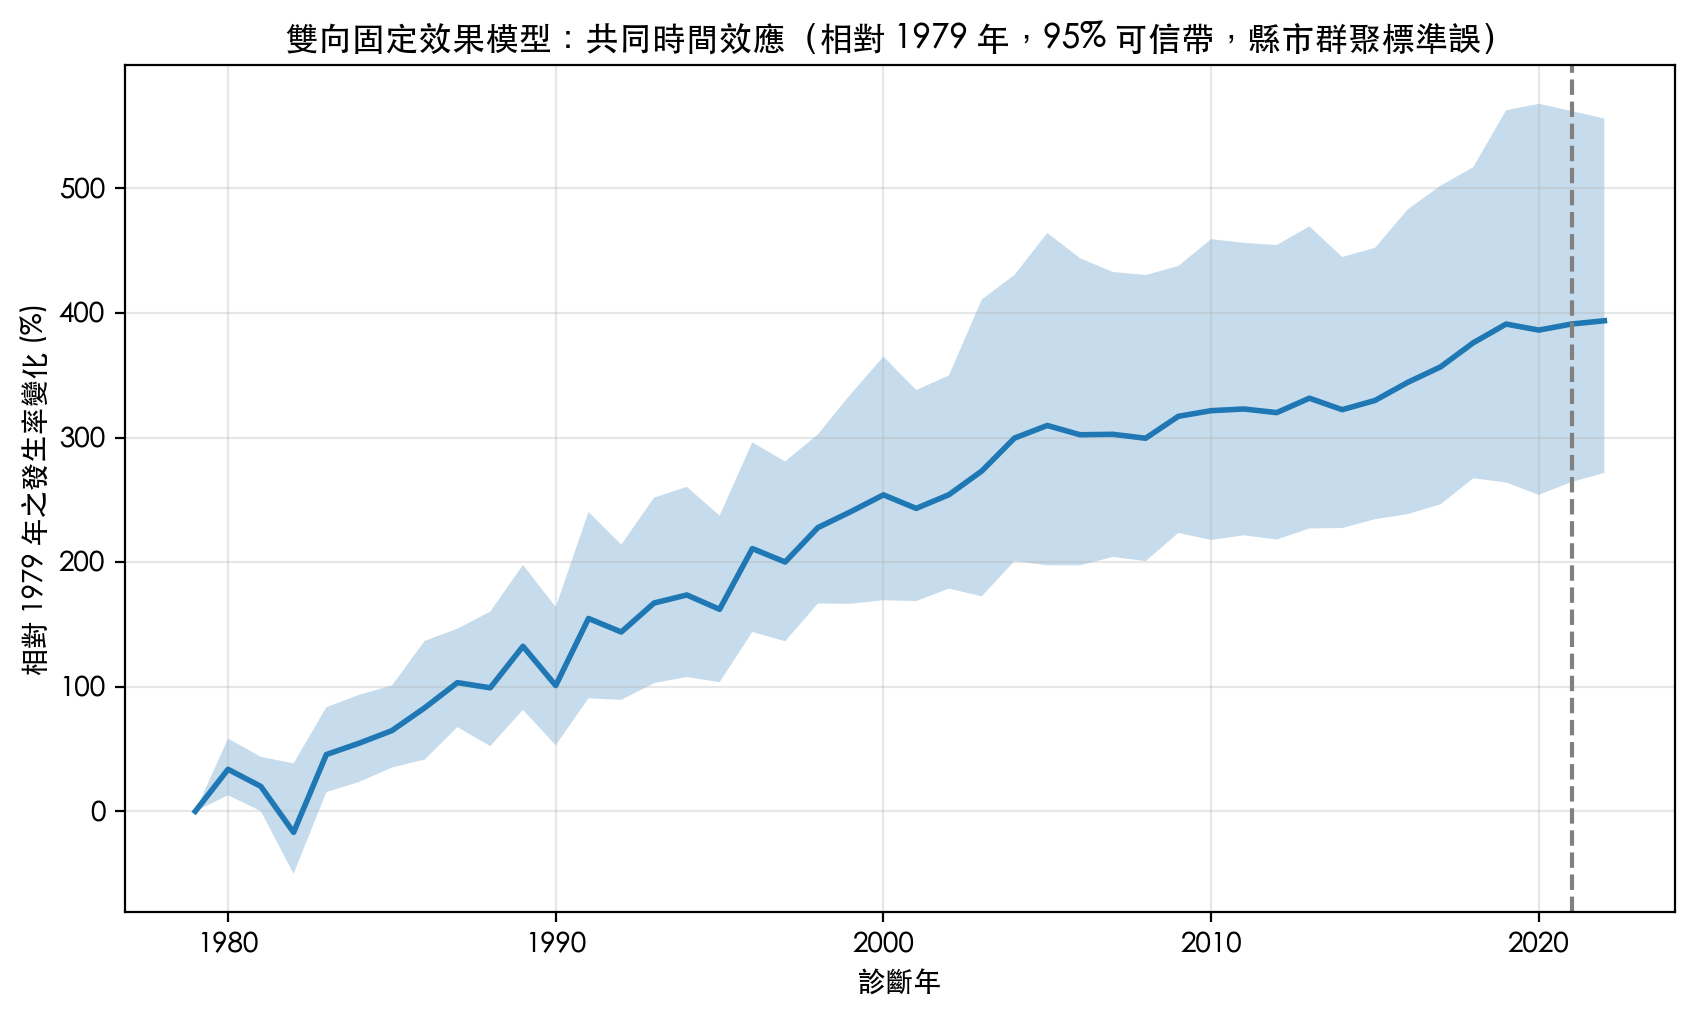
\includegraphics[width=\textwidth]{fe_year_effects.png}\caption{全國共同的年度效應}\end{subfigure}
  \begin{subfigure}{.44\textwidth}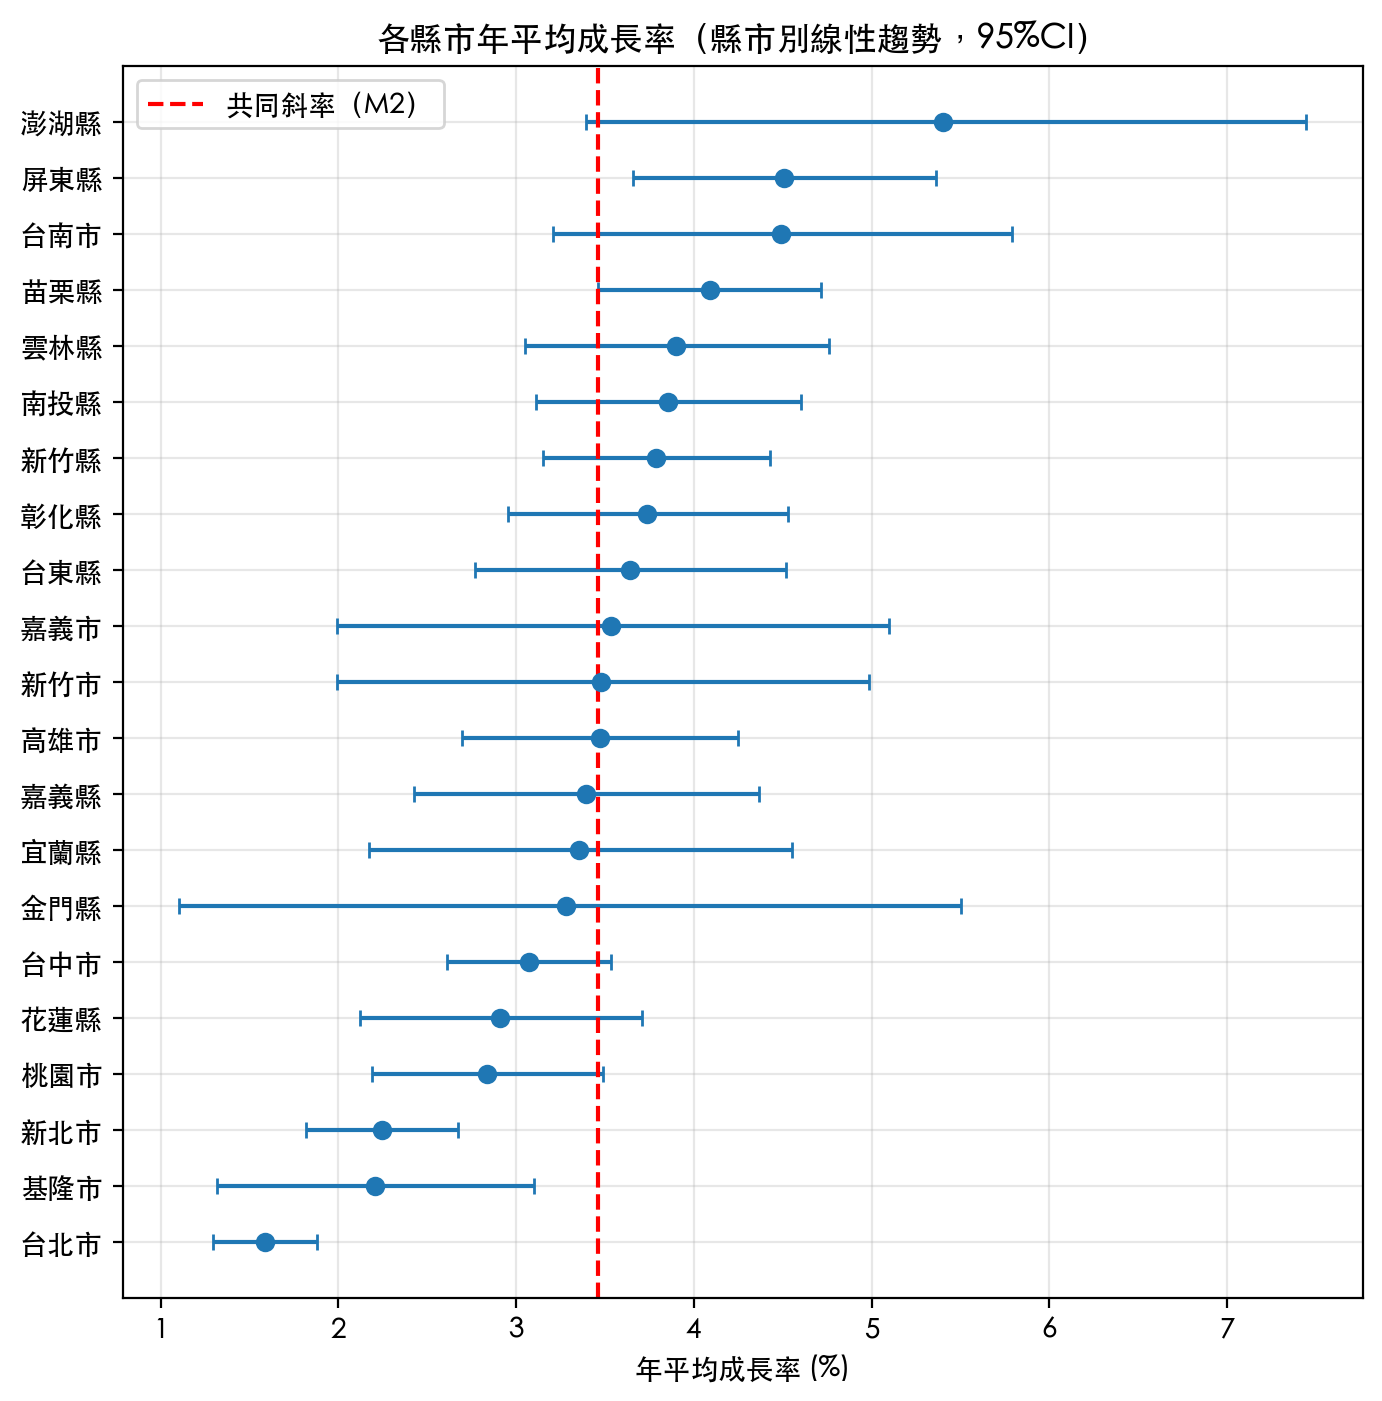
\includegraphics[width=\textwidth]{fe_county_slopes.png}\caption{縣市別年成長率}\label{fig:slopes}\end{subfigure}
  \caption{雙向固定效果的年度效應（相對1979年）與各縣市年成長率。}
\end{figure}

\begin{figure}[H]
  \centering
  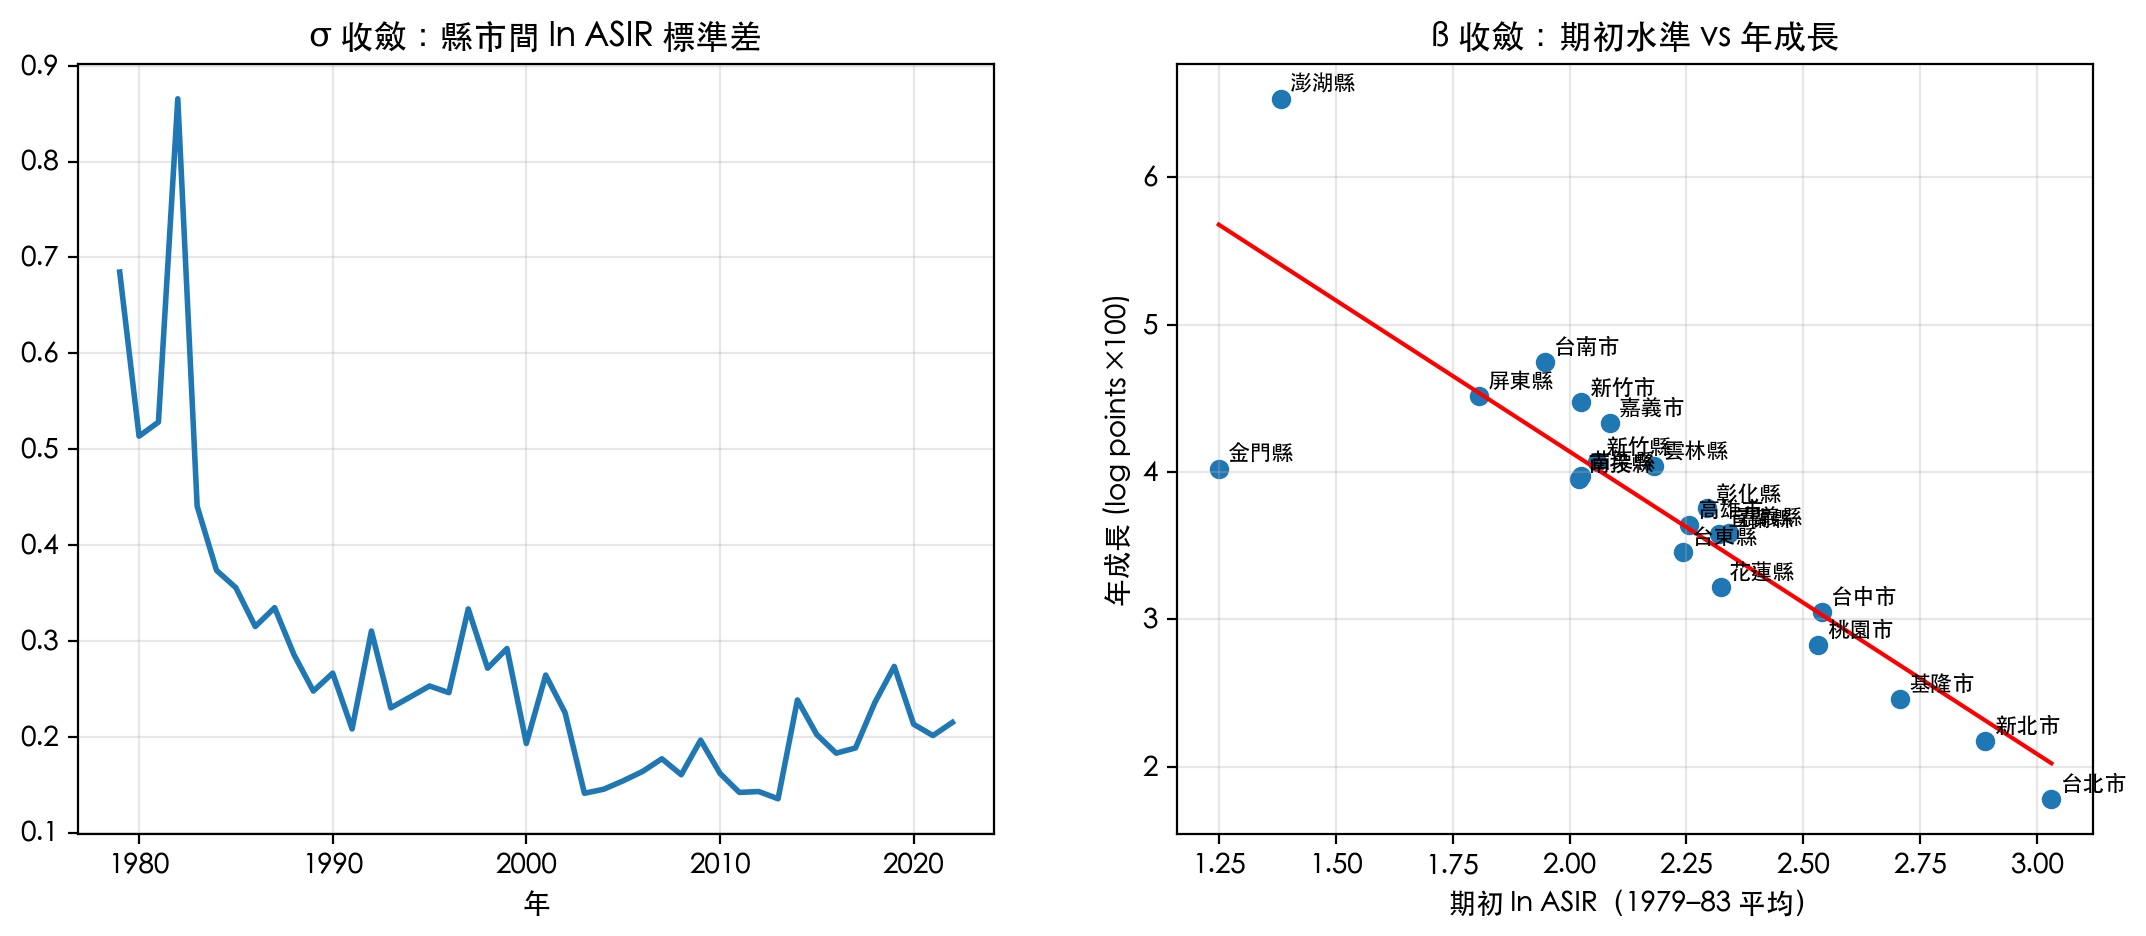
\includegraphics[width=.92\textwidth]{fe_beta_convergence.png}
  \caption{$\sigma$ 收斂（左）與 $\beta$ 收斂（右）。}
\end{figure}

加入時變共變量的雙向固定效果模型（M6）提供的是縣市內部變動的關聯，而不是因果效果。縣市人口的係數為負（$-0.456$，加權後$-0.276$），表示縣市內人口增加的年份，對應的標準化發生率較低；由於本資料沒有年齡別的暴露、移入移出與診斷可近性，這個關聯可能反映人口成長與都會化帶來的組成變化或診斷延遲，不宜解讀為「人口增加使肺癌風險下降」。口腔癌風險代理指標的係數為正（$0.215$，加權後$0.330$）：口腔癌ASIR高的縣市年份，肺癌ASIR也較高，與吸菸、嚼檳榔、飲酒等共同的風險環境一致，但這只是風險代理指標，且兩種癌別有相同的登記與診斷環境，仍屬關聯。

%=====================================================================
\section{疫情衝擊的因果推論}
%=====================================================================
\subsection{雙向固定效果DID與事件研究}
以2009至2022年的縣市面板，估計事件研究設定
\begin{equation}
y_{ct}=\alpha_c+\gamma_t+\sum_{k\neq 2019}\beta_k\,\mathrm{Treat}_c\cdot\mathbf 1[t=k]+\varepsilon_{ct},
\end{equation}
基期為2019年，$\beta_k$（$k\le 2018$）用於檢驗疫情前的平行趨勢，$\beta_{2020},\beta_{2021},\beta_{2022}$為疫情期間的處理效果。表\ref{tab:did}彙整了結果。以雙北為處理組時，疫情後（2021至2022年）的DID估計值為$-1.5\%$（精確隨機化推論 $p=0.80$），2020年為$-5.2\%$（$p=0.42$）；事件研究的年度係數2021年為$-5.2\%$（$p=0.55$）、2022年為$+2.5\%$（$p=0.71$），疫情前的各年係數則都在$\pm4\%$以內且皆不顯著，並未顯示明顯的疫情前趨勢差異。若把處理範圍擴大到北北基桃，疫情後估計為$-5.6\%$（$p=0.27$），2021年為$-9.0\%$（$p=0.18$），方向仍為負但不顯著。加入處理組專屬的線性趨勢以放寬平行趨勢假設後，雙北2021年估計為$-4.0\%$（$p=0.61$），2022年為$+4.0\%$（$p=0.61$）。

\begin{table}[H]
\centering
\caption{DID估計（log points換算為百分比；括號內為精確隨機化推論 $p$ 值）。}\label{tab:did}
\small
\resizebox{\textwidth}{!}{\begin{tabular}{lcccc}
\toprule
設計 & 疫情後(2021--22) & 2020 & 事件研究2021 & 事件研究2022\\
\midrule
雙北 vs 其餘19縣市（210種指派） & $-1.5\%$ (0.80) & $-5.2\%$ (0.42) & $-5.2\%$ (0.55) & $+2.5\%$ (0.71)\\
北北基桃 vs 其餘17縣市（5985種指派） & $-5.6\%$ (0.27) & $-6.3\%$ (0.43) & $-9.0\%$ (0.18) & $-4.4\%$ (0.42)\\
篩檢導向癌別 vs 非篩檢癌別（715種指派） & $-4.2\%$ (0.68) & $-3.8\%$ (0.64) & $-7.2\%$ (0.55) & $-2.2\%$ (0.88)\\
肺癌 vs 非篩檢癌別（10種指派） & $+11.5\%$ (0.60) & $+7.1\%$ (0.90) & $+11.3\%$ (0.80) & $+15.2\%$ (0.60)\\
\bottomrule
\end{tabular}}
\end{table}

\begin{figure}[H]
  \centering
  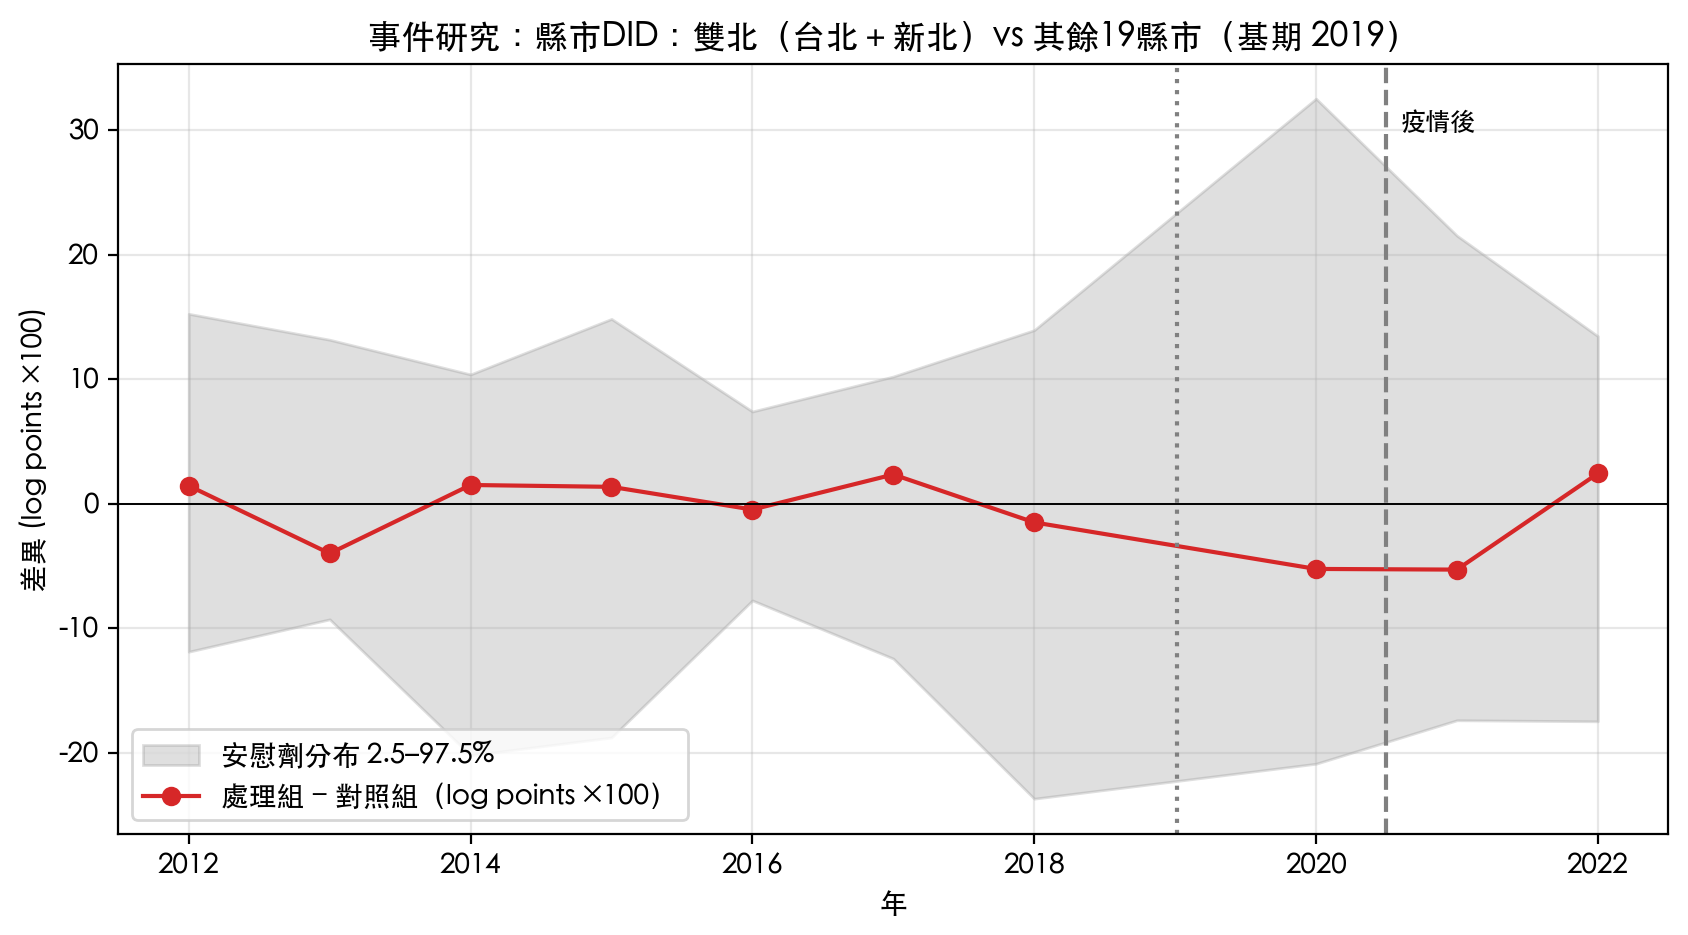
\includegraphics[width=.8\textwidth]{did_event_study_counties_taipei.png}
  \caption{事件研究：雙北 vs 其餘縣市（基期2019；灰色帶為隨機化安慰劑分布的2.5--97.5\%）。}
\end{figure}

這些結果的解讀必須同時看點估計與檢定力。安慰劑分布顯示，在這個設計下，2021年的處理效果即使是$\pm17$至22個對數點（約$\pm16$至24\%）也很容易由隨機的縣市指派產生，意味著本資料只能排除相當大的效應，無法排除幾個百分點的效應。因此「不顯著」不等於「沒有影響」，只是沒有證據顯示影響大到足以在這個樣本中被偵測。

\subsection{敏感度分析：平行趨勢的違反}
事件研究提供了疫情前的偏離量，可以用來衡量結論對平行趨勢違反的容忍度。仿照Rambachan與Roth（2023）的相對大小限制的簡化版本，假設疫情期間的違反幅度不超過疫情前最大偏離的 $M$ 倍。以雙北為例，疫情前最大偏離為0.040個對數點，2021年估計值$-0.053$的「崩潰值」（使區間包含0的最小 $M$）為1.32，2022年估計值$+0.024$的崩潰值為0.61；北北基桃2021年的崩潰值為2.54。換言之，只要疫情期間的趨勢偏離不超過疫情前觀察到的最大偏離的約1.3倍，雙北2021年估計值仍與負向效果相容，但因為這是以點估計為基礎的簡化版本，並未納入抽樣不確定性，需與隨機化推論的結果一併閱讀。

\subsection{合成控制法與增強型合成控制法}
雙北只有兩個處理縣市，合成控制法是處理少數處理單位的標準工具。我們以雙北人口加權的ASIR（取對數）為處理單位，以其餘19個縣市為捐贈池，在2005至2019年配適非負、和為1的權重，使疫情前的軌跡盡可能貼合；另以嶺迴歸偏誤校正的增強型合成控制法（Ben-Michael等，2021）為穩健性檢查。配適良好：疫情前的均方根預測誤差（RMSPE）僅0.0175（約1.8\%）。權重主要落在彰化縣（0.42）、桃園市（0.26）與台南市（0.19），其餘為宜蘭縣、台中市與基隆市。疫情後（2020至2022年）平均而言，雙北實際值相對合成對照高$1.1\%$（$p=0.83$，以19個縣市進行空間安慰劑檢定），增強型合成控制法則為$+0.8\%$（$p=0.67$）；排除可能受外溢影響的基隆與桃園後為$-1.8\%$（$p=0.57$），排除兩個離島後為$+1.1\%$（$p=0.80$）。亦即，不論捐贈池如何設定，雙北相對於「若無疫情」的反事實都沒有可辨識的差距，與DID的結論一致。

\begin{figure}[H]
  \centering
  \begin{subfigure}{.49\textwidth}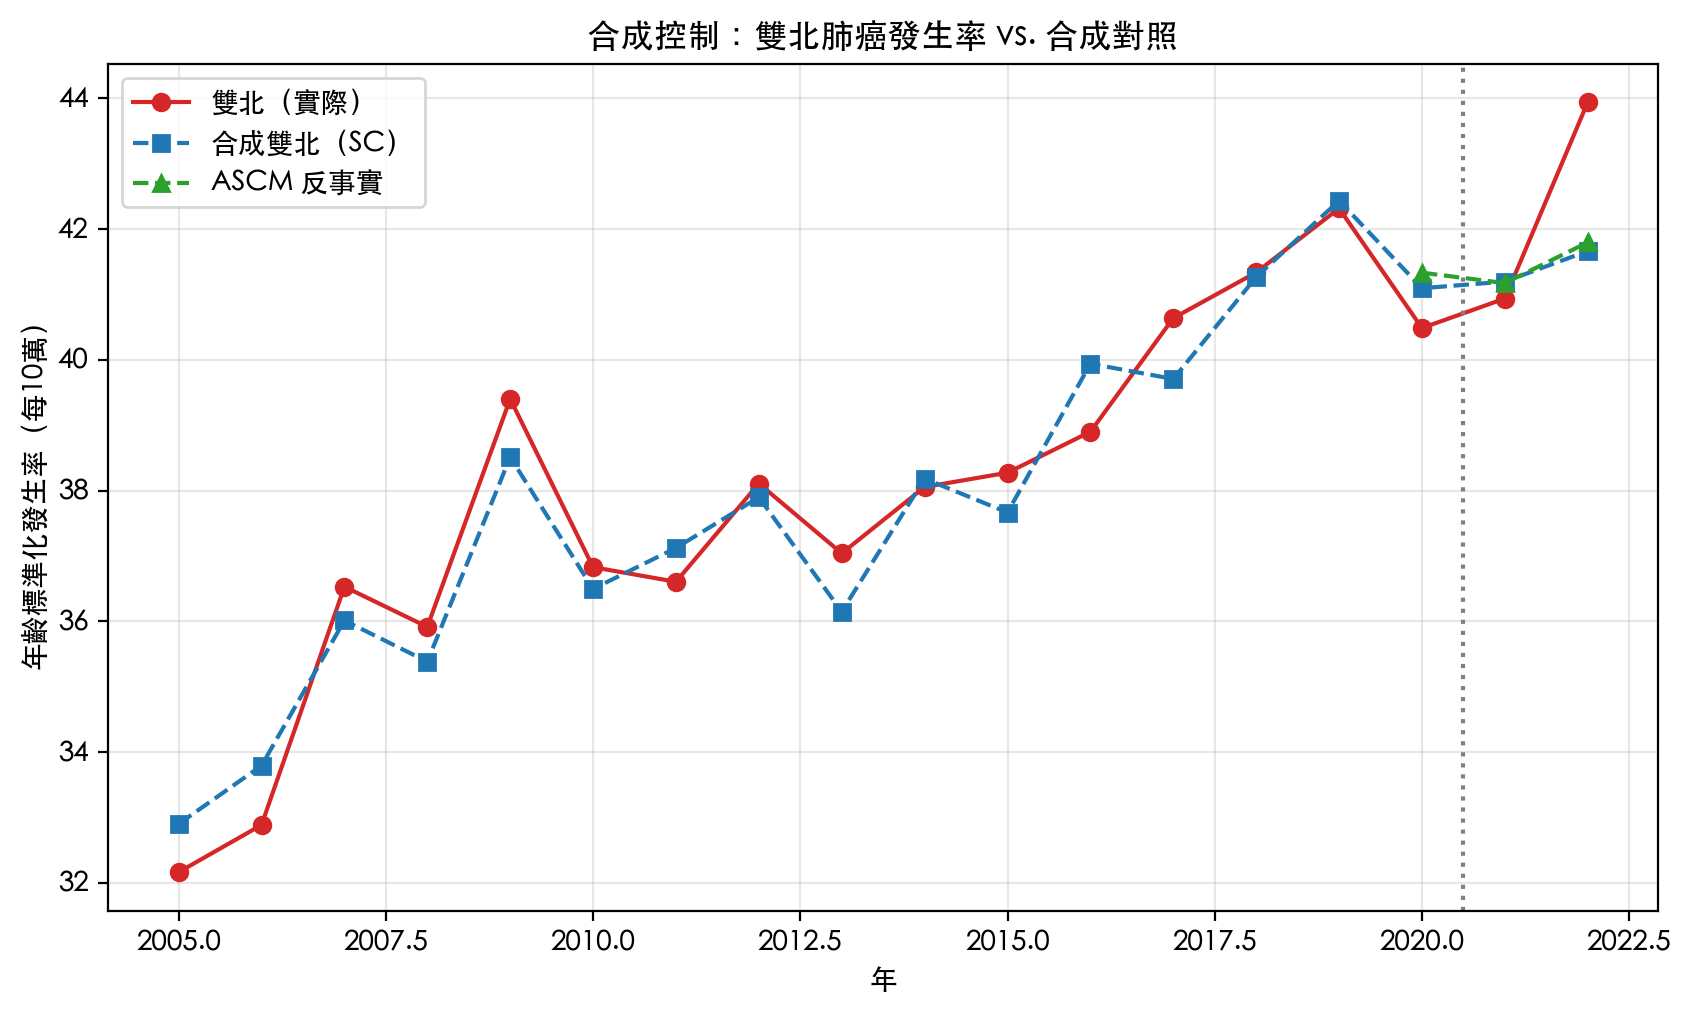
\includegraphics[width=\textwidth]{sc_fit.png}\caption{實際與合成雙北}\end{subfigure}
  \begin{subfigure}{.49\textwidth}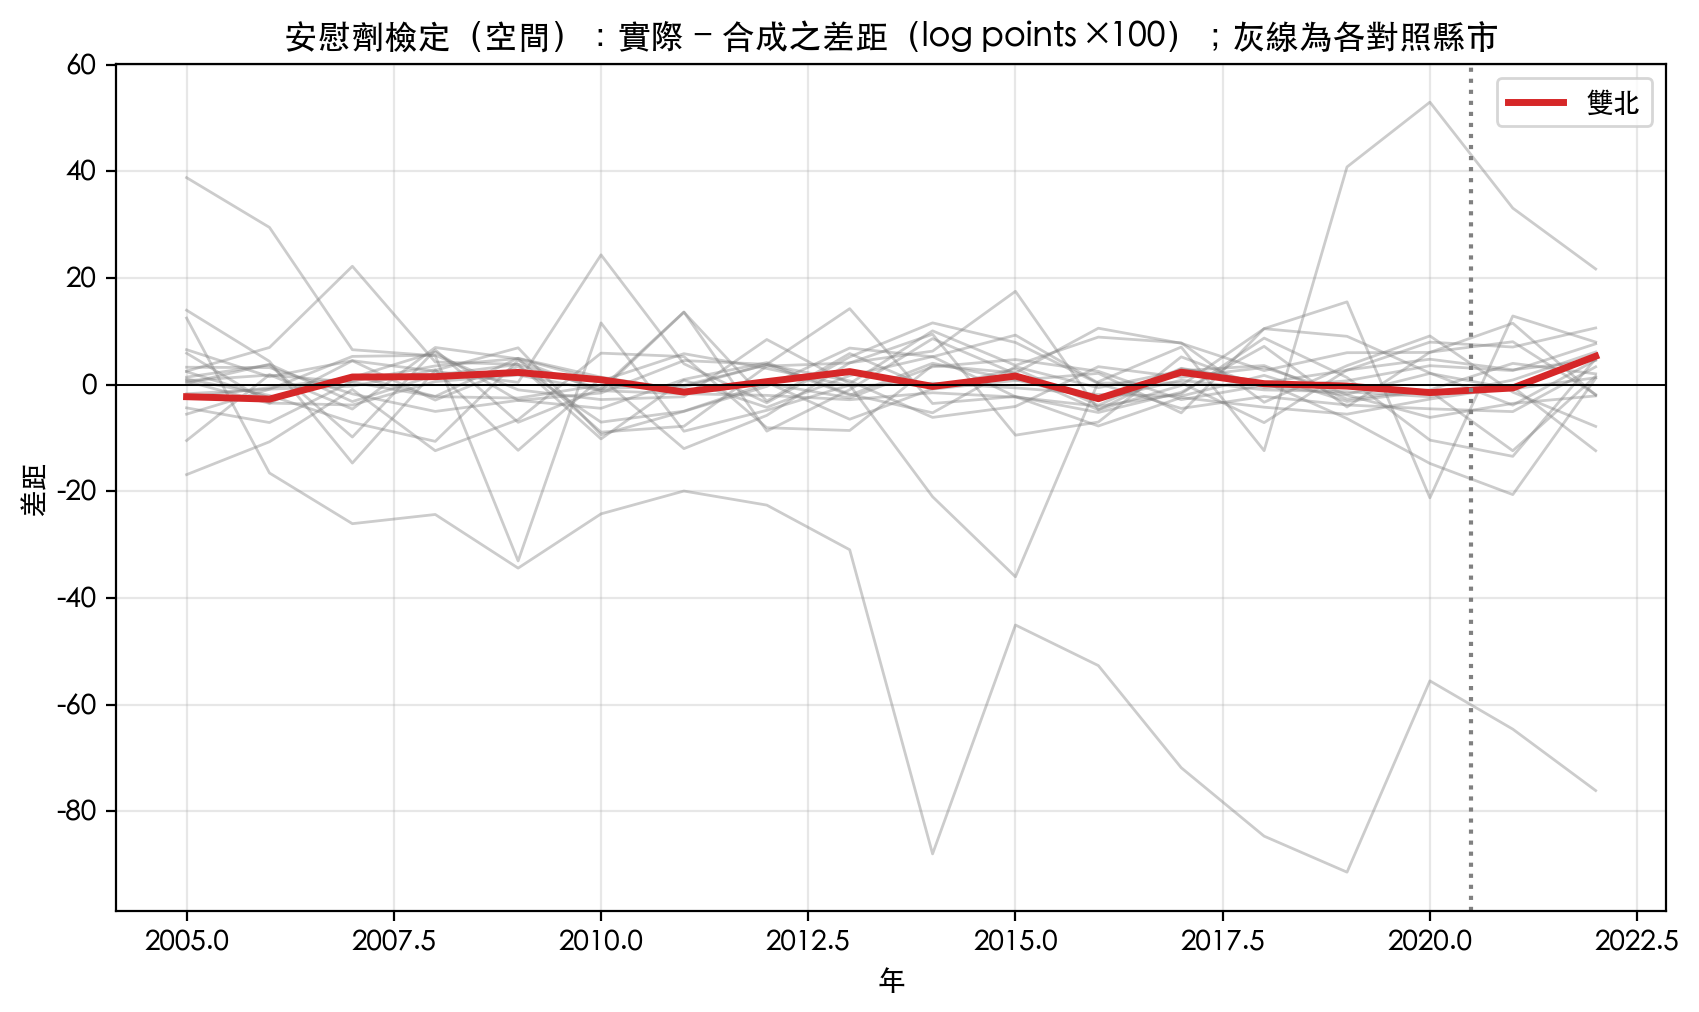
\includegraphics[width=\textwidth]{sc_placebo_gaps.png}\caption{空間安慰劑檢定}\end{subfigure}
  \caption{合成控制：雙北肺癌發生率與合成對照，及各對照縣市的安慰劑差距。}
\end{figure}

\subsection{癌別DID：篩檢導向與非篩檢癌別}
另一個思路是比較癌別：大腸癌、口腔癌、女性乳癌與子宮頸癌屬於國家有組織篩檢的癌別，其被診斷的件數更依賴篩檢活動的持續，若疫情干擾了篩檢，應先反映在這些癌別。以全國的癌別層級面板，比較這四類癌別與九個無國家篩檢計畫的癌別（胃、肝、胰、食道、膀胱、非何杰金氏淋巴瘤、白血病、腦、攝護腺），疫情後的DID估計為$-4.2\%$（715種指派，$p=0.68$），事件研究2021年為$-7.2\%$（$p=0.55$）；方向符合「疫情降低篩檢導向癌別的診斷」的預期，但幅度在隨機化推論下不顯著。肺癌與非篩檢癌別的比較則顯示事件研究的疫情前係數呈上升趨勢（2016年$+5.4\%$、2018年$+9.9\%$），違反平行趨勢，因此疫情後$+11.5\%$的估計不宜解讀為疫情效應；加入處理組專屬趨勢後，2021年與2022年的估計值分別為$-1.4\%$與$+0.4\%$，幾乎為零。

\subsection{雙重機器學習的雙重穩健DID（DML-DiD）}
前面的縣市DID與合成控制法都只有「雙北」這一個處理單位，共變量調整的空間很有限。雙重／去偏機器學習（Chernozhukov等，2018）的想法是：把對共變量的調整交給彈性的機器學習模型，再以Neyman正交化的估計式（使結果對機器學習估計的誤差不敏感）加上交叉配適（cross-fitting，用未參與訓練的資料做預測）取得可靠的處理效果估計。我們把它與DID結合（Sant'Anna與Zhao，2020的雙重穩健DID），分析單位改為「縣市$\times$癌別」的序列：納入21個縣市與28個癌別（扣除個案過少者），共473條序列，其中雙北有56條。結果變數為疫情後（2021、2022或兩年平均）與基期（2017至2019年平均）之間ln ASIR的變化，共變量均為疫情前變數：基期水準、疫情前趨勢（2017--19相對2014--16）、疫情前波動、個案數、縣市人口、癌別與性別。處理效果的估計式有兩種：結果迴歸型（OR-DML）只用對照組配適 $\hat m_0(X)$ 預測「無處理下的變化」，ATT為處理序列的平均殘差；雙重穩健型（DR-DML）再以傾向分數 $\hat\pi(X)$ 加權，只要結果模型或傾向分數模型有一個設定正確即一致。機器學習模型為梯度提升樹（GBM）、隨機森林與Lasso；交叉配適的分組以縣市為單位，使同一縣市的序列不會同時出現在訓練與預測集。

這裡需要強調兩點。第一，處理（雙北）是在縣市層級指派的，而縣市層級只有兩個處理叢集，所以DML的漸近標準誤無法使用；我們對每一個可能的縣市指派（210種）重新執行完整的交叉配適估計，以隨機化推論的 $p$ 值為準。第二，這個估計量的估計對象與前面不同：它是雙北「所有癌別平均」的診斷變化，反映的是疫情對診斷與登記體系的整體衝擊；肺癌只是其中2條序列，因此另以異質性分析檢視肺癌、篩檢導向癌別與其他癌別。

結果（表\ref{tab:dml}）顯示，不論機器學習模型與估計式為何，疫情後的ATT都接近零：以GBM的OR-DML估計為$+1.0\%$（隨機化推論 $p=0.64$）、DR-DML為$+1.4\%$（$p=0.52$）；以Lasso則為$-1.7\%$（$p=0.40$）與$-0.8\%$（$p=0.68$）；隨機森林的點估計為$+1.0\%$與$+0.9\%$。未經共變量調整的DID為$+2.0\%$，表示調整使估計值略往零靠近。分年份來看，2021年的ATT為$-0.8\%$至$-2.0\%$（$p=0.53$至0.77），2022年為$+0.1\%$至$+3.4\%$，2020年為$-3.7\%$至$+1.3\%$，皆不顯著。與縣市DID相比最重要的差別在檢定力：因為結果是28個癌別的平均，安慰劑分布的標準差只有約0.02至0.03個對數點，2.5至97.5百分位約為$\pm 4$至$6$個對數點，遠小於縣市DID的$\pm 17$至22個對數點。換言之，疫情對雙北整體癌症診斷的平均影響若大於約5\%，這個設計很可能已經偵測到；沒有偵測到，說明整體診斷體系的衝擊相當有限。

異質性分析（表\ref{tab:dml}下半）顯示，肺癌的ATT為$-1.9\%$（$p=0.66$；僅2條序列，安慰劑標準差0.054，估計很不精確），篩檢導向癌別為$-2.4\%$（8條序列，$p=0.50$），其他癌別為$-1.5\%$（46條序列，$p=0.52$）。篩檢導向癌別的點估計略低，方向與篩檢中斷的預期一致，但與其他癌別的差距遠小於隨機波動。逐癌別的ATT範圍很大（由喉癌的$-13\%$到何杰金氏淋巴瘤的$+27\%$），但單一癌別在雙北只有一至兩條序列，個案數少，這些數字只是雜訊的展現，不宜個別解讀（圖\ref{fig:dmlsite}）。事前安慰劑檢定（假裝疫情發生在2017或2018年）得到$-1.2\%$（$p=0.52$）與$+0.1\%$（$p=0.96$），沒有出現虛假的處理效果，支持以疫情前趨勢及共變量調整後的平行趨勢假設。

\begin{table}[H]
\centering
\caption{DML-DiD的ATT估計（473條縣市$\times$癌別序列；log points換算為百分比；括號內為210種指派的隨機化推論 $p$ 值）。}\label{tab:dml}
\small
\begin{tabular}{lcccc}
\toprule
學習器／估計式 & 2020 & 2021 & 2022 & 2021--22\\
\midrule
GBM, OR-DML & $+0.2$ (--) & $-0.8$ (0.74) & $+2.1$ (--) & $+1.0$ (0.64)\\
GBM, DR-DML & $+1.3$ (--) & $-0.8$ (0.77) & $+3.4$ (--) & $+1.4$ (0.52)\\
Lasso, OR-DML & $-3.7$ (--) & $-1.6$ (0.60) & $+0.1$ (--) & $-1.7$ (0.40)\\
Lasso, DR-DML & $-2.4$ (--) & $-2.0$ (0.53) & $+1.7$ (--) & $-0.8$ (0.68)\\
隨機森林, OR-DML／DR-DML & $+0.1$／$+0.8$ & $-0.5$／$-0.1$ & $+2.6$／$+2.3$ & $+1.0$／$+0.9$\\
未調整DID（序列平均） & -- & -- & -- & $+2.0$\\
\midrule
\multicolumn{5}{l}{異質性（Lasso, OR-DML, 2021--22）：癌別群 ATT (RI $p$)}\\
肺癌（2條序列） & \multicolumn{4}{l}{$-1.9\%$ (0.66)}\\
篩檢導向癌別（8條序列） & \multicolumn{4}{l}{$-2.4\%$ (0.50)}\\
其他癌別（46條序列） & \multicolumn{4}{l}{$-1.5\%$ (0.52)}\\
事前安慰劑（GBM, OR-DML） & \multicolumn{4}{l}{假設疫情在2017年：$-1.2\%$ (0.52)；2018年：$+0.1\%$ (0.96)}\\
\bottomrule
\end{tabular}
\end{table}

\begin{figure}[H]
  \centering
  \begin{subfigure}{.62\textwidth}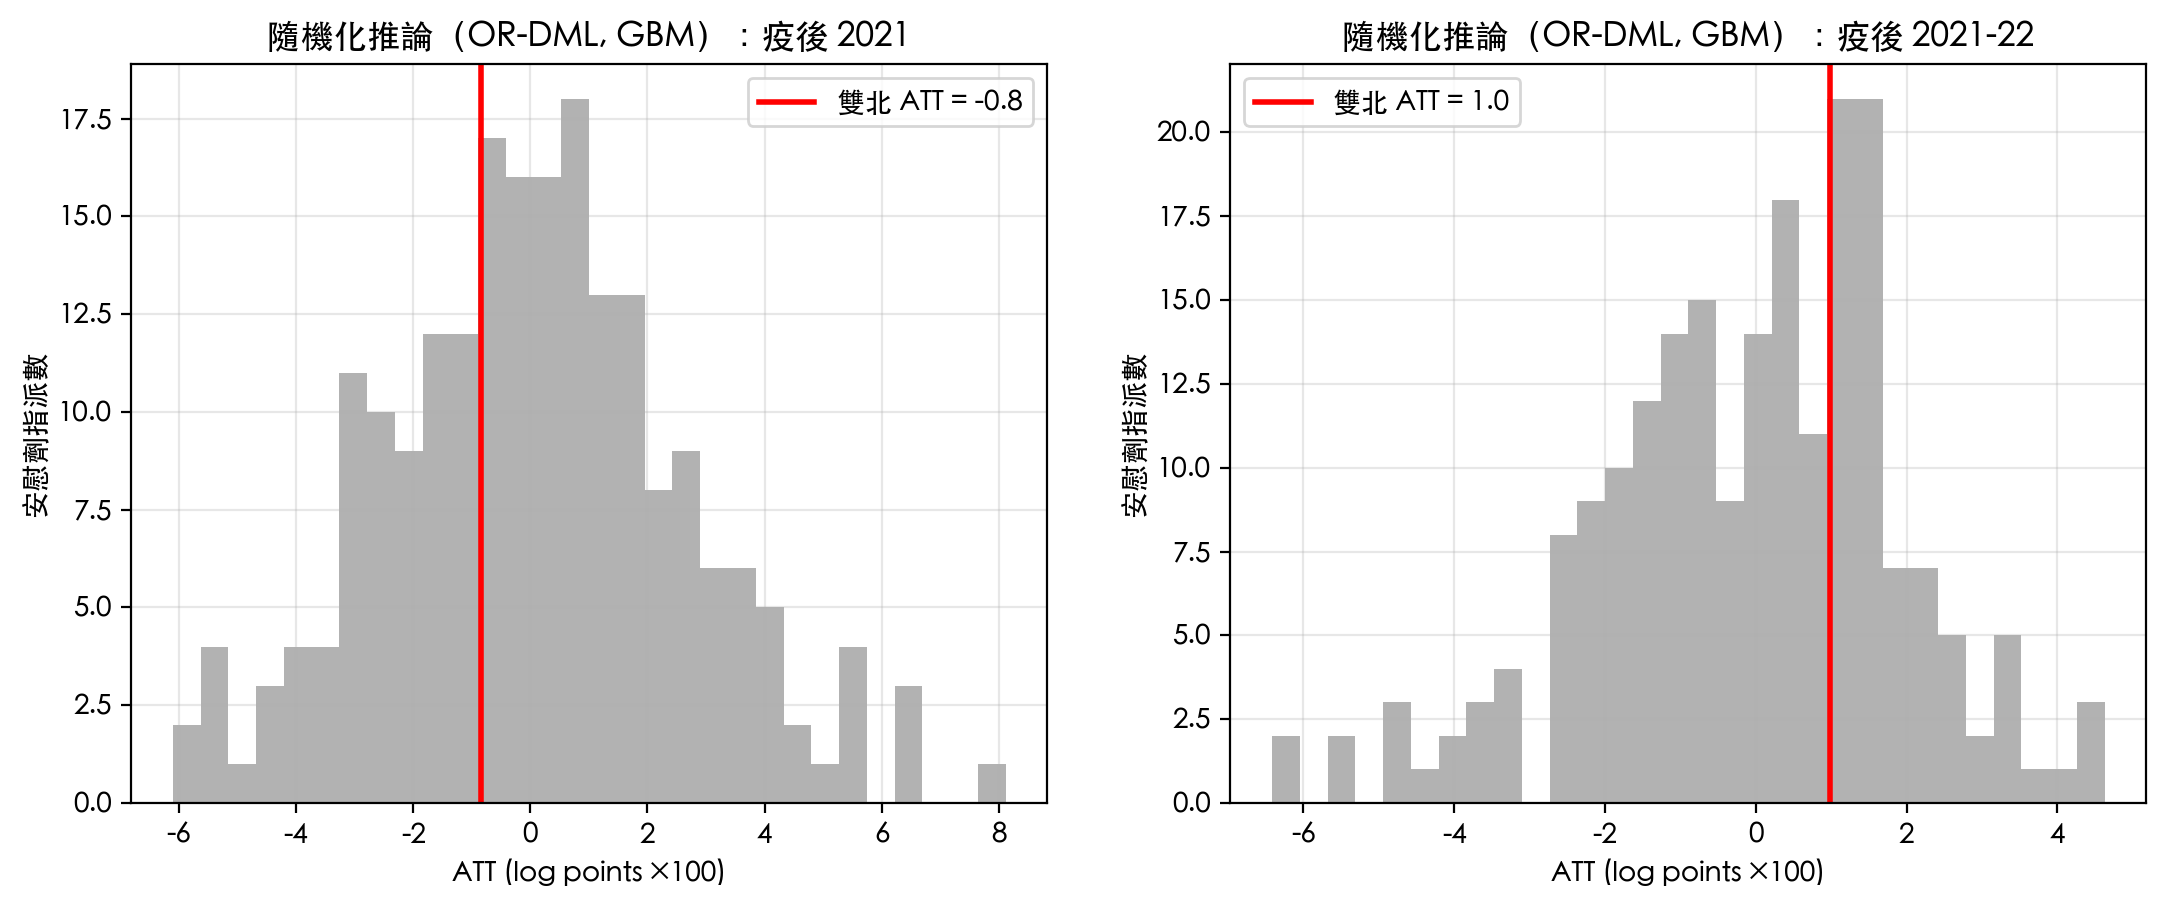
\includegraphics[width=\textwidth]{dml_ri_distribution.png}\caption{隨機化推論分布（GBM, OR-DML）}\end{subfigure}
  \begin{subfigure}{.36\textwidth}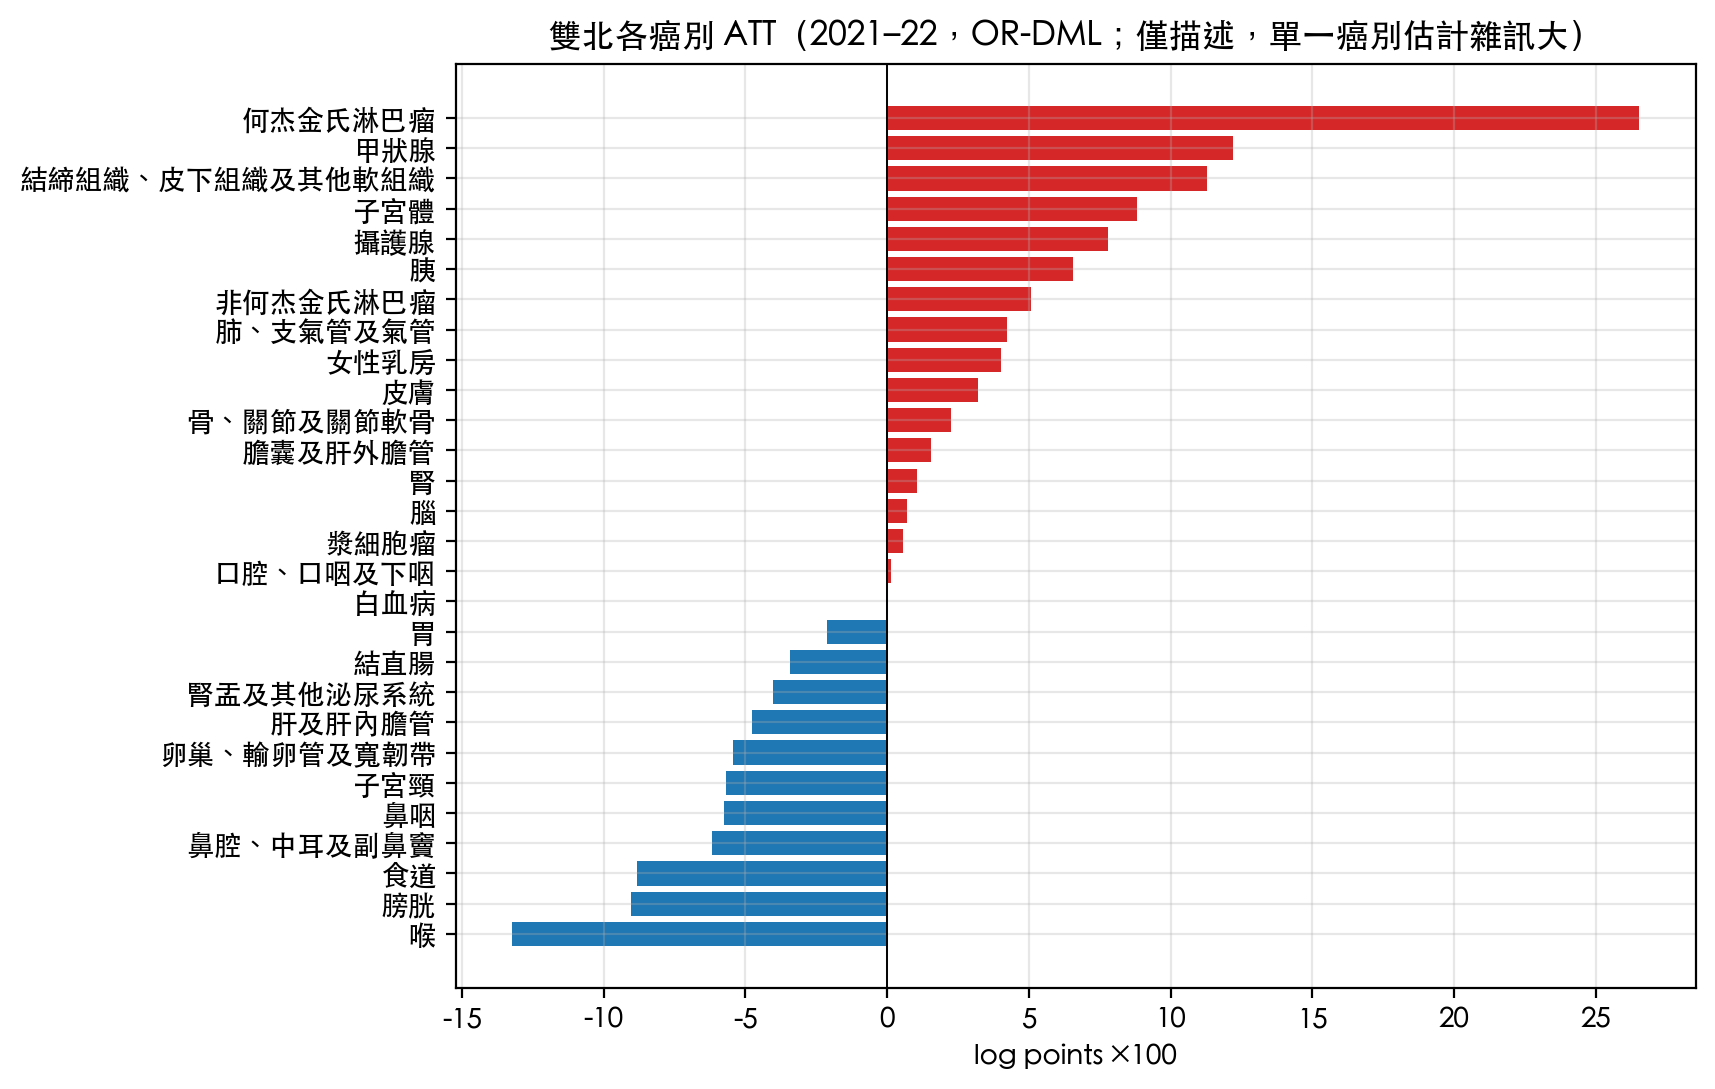
\includegraphics[width=\textwidth]{dml_did_by_site.png}\caption{雙北各癌別ATT（描述性）}\label{fig:dmlsite}\end{subfigure}
  \caption{DML-DiD：觀察到的ATT（紅線）相對於所有安慰劑指派的分布，及逐癌別估計。}
\end{figure}


\subsection{因果推論的小結}
把幾種方法並列可以看出一致的圖像（表\ref{tab:causal}）：雙北肺癌發生率相對於反事實在疫情期間的變化，估計值介於$-5\%$與$+1\%$之間，方向不一致、都不顯著；以全癌別平均的DML-DiD估計也接近零（$-1.7\%$至$+1.4\%$）；篩檢導向癌別的下降較大（約$-4\%$至$-7\%$），但同樣沒有統計顯著性。這個結論的力量主要來自「多種方法收斂到同一個結論」，而不是任何單一方法的精確度；其限制則在於處理單位太少，所有方法的檢定力都有限。

\begin{table}[H]
\centering
\caption{不同因果推論方法對雙北疫情後肺癌發生率變化的估計。}\label{tab:causal}
\small
\begin{tabular}{lcc}
\toprule
方法 & 估計（\%） & 隨機化／安慰劑 $p$\\
\midrule
TWFE DID（雙北，2021--22） & $-1.5$ & 0.80\\
TWFE DID（北北基桃，2021--22） & $-5.6$ & 0.27\\
合成控制法（2020--22平均） & $+1.1$ & 0.83\\
增強型合成控制法 & $+0.8$ & 0.67\\
DML-DiD（全癌別平均；GBM, OR-DML，2021--22） & $+1.0$ & 0.64\\
DML-DiD（全癌別平均；Lasso, DR-DML，2021--22） & $-0.8$ & 0.68\\
\bottomrule
\end{tabular}
\end{table}

%=====================================================================
\section{健康不平等與空間自回歸模型}
%=====================================================================
\subsection{不平等的趨勢：相對與絕對}
健康經濟學區分相對不平等與絕對不平等，因為兩者可能走向相反的方向。我們計算人口加權的Gini係數與Theil指數、變異係數、$P_{90}/P_{10}$比值作為相對指標，以標準差與全距作為絕對指標，並以縣市人口規模的名次（ridit）為排序，估計斜率不平等指數（SII）、相對不平等指數（RII）與集中指數；這裡以人口規模作為都會規模梯度的代理，並非社經地位的排序（本資料沒有所得或教育變數）。表\ref{tab:ineq}顯示，相對不平等大幅下降：變異係數由1979年的0.61降至2022年的0.16，人口加權Gini由0.294降至0.045，Theil由0.143降至0.004，RII由0.83降至0.10。但絕對離散並沒有隨之縮小：縣市間ASIR的標準差在1979年為5.8，2022年為6.5，且在2019年達8.5（主要受澎湖縣高峰影響）；全國平均發生率由10.7上升至41.7，同樣的相對差距對應的絕對差距因此變大。SII則在1980年代初達高峰（1981年為13.7），1989年為11.0，其後下降至2019年的2.3與2022年的4.3，表示依人口規模排序的絕對落差已大幅縮小。

這個結果的政策意涵是：若以相對指標評估，縣市間的肺癌發生率差距已幾乎消失；但若考慮絕對的疾病負擔，各縣市之間仍相差數個至十餘個每十萬人，而且整體疾病負擔已增加三倍以上。相對指標下降的原因，部分來自所有縣市同時被抬升到較高的基準，而不是高發縣市降低。

\begin{table}[H]
\centering
\caption{不平等指標（人口加權；每10萬人口）。}\label{tab:ineq}
\small
\begin{tabular}{lrrrrrr}
\toprule
指標 & 1979 & 1989 & 1999 & 2009 & 2019 & 2022\\
\midrule
加權平均 ASIR & 10.7 & 20.6 & 30.8 & 36.2 & 40.9 & 41.7\\
標準差（絕對） & 5.84 & 4.49 & 6.50 & 6.15 & 8.51 & 6.53\\
變異係數（相對） & 0.608 & 0.237 & 0.233 & 0.183 & 0.212 & 0.164\\
Gini（加權） & 0.294 & 0.126 & 0.081 & 0.068 & 0.045 & 0.045\\
Theil（加權） & 0.143 & 0.025 & 0.011 & 0.008 & 0.005 & 0.004\\
SII（絕對；人口規模梯度） & 8.95 & 10.97 & 8.56 & 6.40 & 2.29 & 4.26\\
RII（相對） & 0.834 & 0.532 & 0.278 & 0.177 & 0.056 & 0.102\\
\bottomrule
\end{tabular}
\end{table}

\begin{figure}[H]
  \centering
  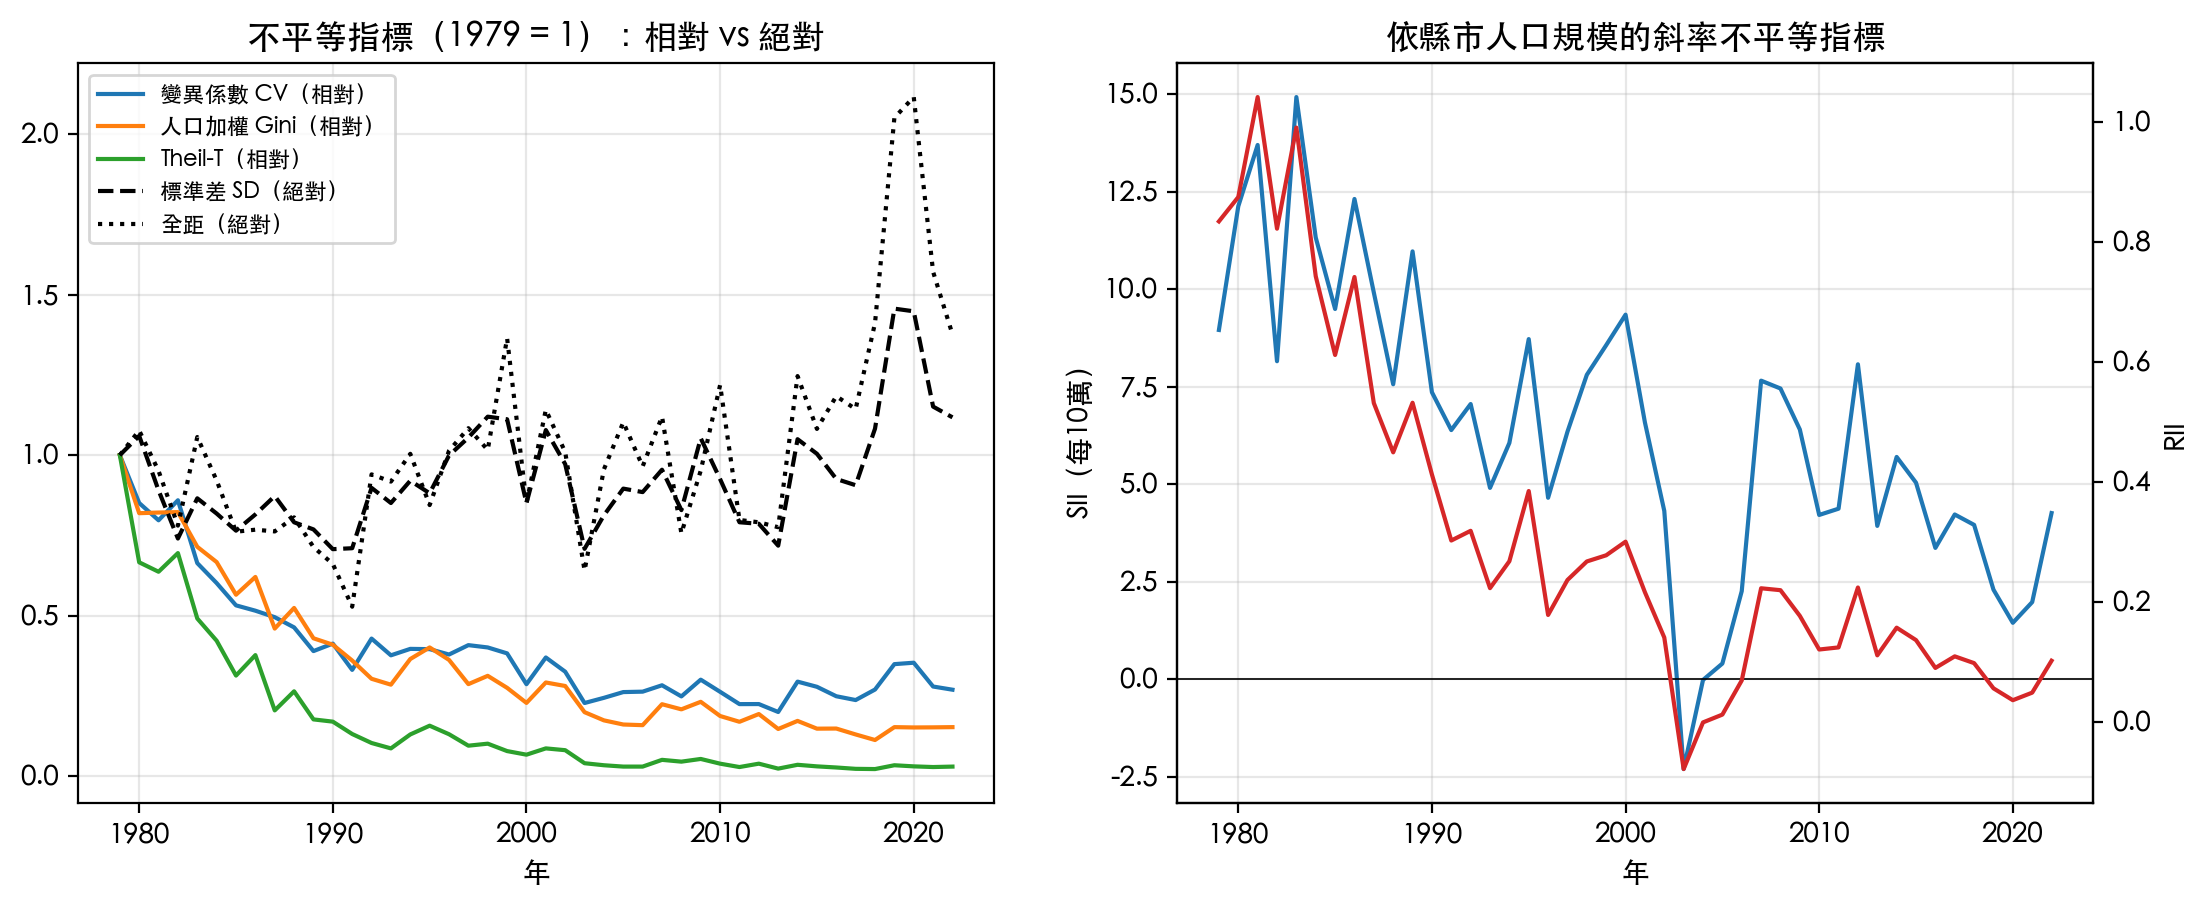
\includegraphics[width=\textwidth]{ineq_trends.png}
  \caption{相對與絕對不平等指標（左，1979年=1），及依人口規模的SII與RII（右）。}
\end{figure}

\subsection{空間自回歸模型}
為檢驗縣市之間是否仍存在空間相互依賴，我們以五年為一個窗口（1979--83、1984--88、$\dots$、2014--18與2019--22共9個），對各窗口縣市平均ASIR的對數做橫斷面空間迴歸，空間權重為列標準化的queen鄰接矩陣（離島以最近縣市連結，見主報告），並以4最近鄰權重作穩健性檢查。模型包括空間滯後（SAR）$y=\rho Wy+X\beta+\varepsilon$ 與空間誤差（SEM）$y=X\beta+u,\ u=\lambda Wu+\varepsilon$，以最大概似法估計（對 $\rho$ 或 $\lambda$ 做集中概似），依Anselin等（1996）計算LM-lag、LM-error及其穩健版本，並檢定殘差的Moran's $I$；共變量為ln人口。由於僅有21個觀察值，我們以概似比檢定（LR）為主要推論依據。

表\ref{tab:sar}顯示空間依賴的消退。1979至1983年SAR的 $\rho=0.55$（LR檢定 $p=0.016$），殘差Moran's $I=0.28$（$p=0.03$），LM-lag檢定 $p=0.029$ 而LM-error檢定 $p=0.12$，依Anselin的決策準則較支持空間滯後型態，也就是一個縣市的發生率與其鄰近縣市的發生率相互影響（較可能反映擴散與共同的區域暴露，如都會區的早期吸菸盛行與就醫環境）。1989至1993年 $\rho=0.48$（$p=0.047$）仍顯著，之後各窗口的 $\rho$ 降為0.27至0.28、接近0甚至為負：2014至2018年 $\rho\approx 0$（$p=0.999$），2019至2022年 $\rho=-0.61$（$p=0.06$）。後者的負值需要謹慎：它受到少數極端值（澎湖的高峰、金門的低值）與離島人為鄰接設定的強烈影響，不宜解讀為真實的「負向空間溢出」。以4最近鄰權重得到的結論相同：1979至1983年 $\rho=0.57$（$p=0.056$）、2014至2018年 $\rho=0.02$（$p=0.97$）。加入口腔癌風險代理指標後，1979至1983年的 $\rho$ 為0.64（$p=0.003$），共變量解釋了部分但並未消除空間依賴。

縣市人口的彈性在1979至1983年最大（OLS 0.24，SAR 0.19），表示當時人口規模越大的縣市發生率越高（都會梯度），此後降至0.03至0.09，與前述SII與RII的下降一致。

\begin{table}[H]
\centering
\caption{各窗口空間迴歸結果（queen權重；因變數 $\ln$ ASIR；共變量 ln人口；$p$ 為概似比或LM檢定）。}\label{tab:sar}
\small
\resizebox{\textwidth}{!}{\begin{tabular}{lcccccc}
\toprule
窗口 & 殘差Moran's $I$ ($p$) & SAR $\rho$ ($p_{LR}$) & SEM $\lambda$ ($p_{LR}$) & LM-lag $p$ & LM-err $p$ & ln人口（OLS/SAR）\\
\midrule
1979--83 & 0.276 (0.03) & 0.548 (0.016) & 0.582 (0.042) & 0.029 & 0.12 & 0.24 / 0.19\\
1984--88 & 0.210 (0.07) & 0.386 (0.12) & 0.389 (0.17) & 0.14 & 0.24 & 0.09 / 0.07\\
1989--93 & 0.303 (0.02) & 0.477 (0.047) & 0.476 (0.063) & 0.053 & 0.09 & 0.05 / 0.03\\
1994--98 & 0.126 (0.14) & 0.277 (0.28) & 0.252 (0.40) & 0.30 & 0.48 & 0.07 / 0.06\\
1999--03 & 0.120 (0.16) & 0.273 (0.27) & 0.236 (0.43) & 0.29 & 0.50 & 0.09 / 0.08\\
2004--08 & $-0.056$ (0.49) & $-0.075$ (0.78) & $-0.093$ (0.74) & 0.79 & 0.76 & 0.03 / 0.03\\
2009--13 & 0.131 (0.13) & 0.261 (0.31) & 0.261 (0.39) & 0.34 & 0.46 & 0.06 / 0.06\\
2014--18 & $-0.026$ (0.43) & $-0.000$ (1.00) & $-0.073$ (0.84) & 1.00 & 0.88 & 0.09 / 0.09\\
2019--22 & $-0.237$ (0.92) & $-0.611$ (0.06) & $-0.610$ (0.07) & 0.17 & 0.18 & 0.05 / 0.05\\
\bottomrule
\end{tabular}}
\end{table}

\begin{figure}[H]
  \centering
  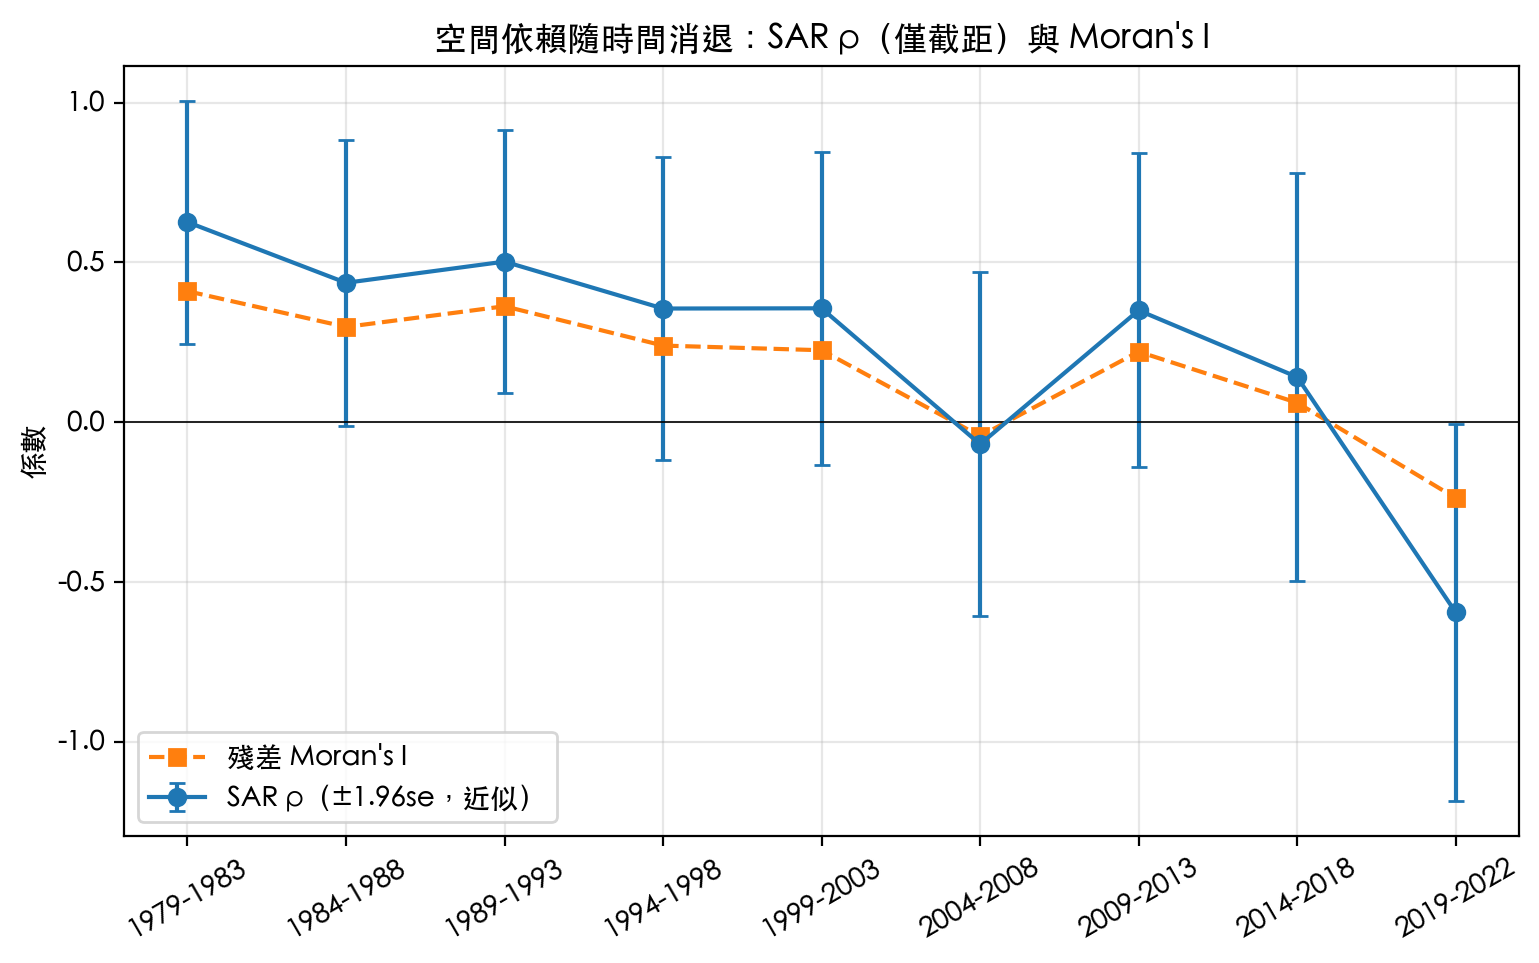
\includegraphics[width=.72\textwidth]{sar_rho_by_window.png}
  \caption{空間依賴隨時間消退：SAR $\rho$（僅截距模型，$\pm1.96$ 標準誤為近似值）與殘差Moran's $I$。}
\end{figure}

最後檢驗收斂是否具有空間成分。以1979--83至2018--22的年成長率對期初水準迴歸，並加入空間滯後項，$\beta$收斂係數在OLS為$-0.0194$、SAR為$-0.0186$（$\rho=0.08$，$p=0.70$；加入ln人口後為$-0.0214$與$-0.0206$），4最近鄰權重的結果相同。換言之，$\beta$收斂並未被空間依賴所解釋，追趕的現象主要是縣市自身水準的函數；不過成長率本身仍有空間相關（Moran's $I=0.41$），穩健LM檢定在queen權重下偏向空間誤差型態（$p\approx 0.05$），表示存在未納入模型的、有空間結構的共同因素。

%=====================================================================
\section{討論}
%=====================================================================
本文的三組結果可以串成一個關於疾病負擔、衝擊與不平等的故事。第一，肺癌的疾病負擔在四十餘年間以每年約3.4\%的速度成長，各縣市的速度不同，後發縣市追趕較快，使縣市間的相對差距在1980年代快速縮小。這提示衛生支出的預測不應只看全國平均：成長最快的是屏東、台南與澎湖等縣市，它們需要的醫療與篩檢資源增幅會高於已進入高原期的雙北。第二，從因果推論的角度，2021年的本土疫情並沒有在雙北留下可偵測的肺癌發生率變化，這與肺癌診斷主要由症狀驅動、較不依賴常規篩檢的特性相符：與大腸癌、乳癌等有組織篩檢的癌別相比，肺癌在疫情期間的診斷較不易因篩檢中斷而減少。這也暗示，在2022年7月國民健康署開始推動低劑量電腦斷層（LDCT）篩檢之後\note{請核對方案起訖與對象條件}，未來的發生率將更依賴篩檢的持續，對類似疫情衝擊會更為敏感，值得持續監測。第三，從不平等的角度，相對不平等已幾乎消失而且空間依賴也已消退，但絕對的疾病負擔增加，並且存在小人口縣市極端波動的風險。以區域為單位的資源配置在1980至1990年代是合理的（空間依賴顯著），但如今風險已散布各地，更適合以縣市甚至更細的單位，依疾病負擔、診斷期別與存活等指標進行目標性介入。

方法上，本文的結果也呈現幾個教訓。處理組只有兩個縣市時，隨機化推論比叢集穩健標準誤可信，但檢定力有限，所以「不顯著」必須與「最小可偵測效應」一併報告；合成控制法與DID使用不同的反事實假設，得到一致的結論，比任何單一方法更有說服力；至於機器學習的角色，雙重機器學習提供的是「在高維度共變量下，穩健地調整已觀察的混雜因素」，並不能彌補處理單位過少或未觀察混雜的問題，這也是本文把DML與隨機化推論結合使用的原因。

%=====================================================================
\section{研究限制}
%=====================================================================
首先，資料沒有縣市別的疫情暴露強度，我們只能依雙北為疫情核心的事實作二分設計，這會使處理組內部的差異被忽略（例如雙北內各行政區的暴露差異），也使「處理」包含了封城、就醫行為改變與篩檢中斷等多種機制，無法拆解。其次，只有兩個處理縣市，所有的推論都建立在隨機化推論之上，其前提是處理指派在縣市之間可交換，而雙北與其他縣市在人口規模、都市化程度上顯著不同，這個前提只能近似成立。第三，疫情後的觀察期僅有三年（2020至2022年），且2022年全國均受Omicron疫情影響，使對照組也受到處理，DID的估計因此偏向零；若有後續年度的資料，應延長觀察期。第四，登記資料以診斷年為準，疫情造成的診斷延遲可能把個案推遲到後續年度，而非真正減少，因此即使2021年發生率下降，也不一定代表疾病負擔減少。第五，固定效果模型中的人口與口腔癌係數僅是關聯，並非因果效果，且缺少所得、教育、醫療資源與吸菸率等決定因素；SAR模型亦僅有21個觀察值，漸近理論下的推論需謹慎。最後，本文的癌別DID以全國層級資料建立，分類（篩檢導向與非篩檢）是依政策認定，同一癌別內部（如早期與晚期）的差異無法分辨。

%=====================================================================
\section*{參考文獻}
%=====================================================================
\begin{small}
\begin{thebibliography}{99}
  \bibitem{r1} Abadie A, Diamond A, Hainmueller J. Synthetic control methods for comparative case studies: estimating the effect of California's tobacco control program. \emph{J Am Stat Assoc}. 2010;105(490):493--505.
  \bibitem{r2} Anselin L, Bera AK, Florax R, Yoon MJ. Simple diagnostic tests for spatial dependence. \emph{Reg Sci Urban Econ}. 1996;26(1):77--104.
  \bibitem{r3} Arkhangelsky D, Athey S, Hirshberg DA, Imbens GW, Wager S. Synthetic difference-in-differences. \emph{Am Econ Rev}. 2021;111(12):4088--4118.
  \bibitem{r4} Ben-Michael E, Feller A, Rothstein J. The augmented synthetic control method. \emph{J Am Stat Assoc}. 2021;116(536):1789--1803.
  \bibitem{r5} Chernozhukov V, Chetverikov D, Demirer M, Duflo E, Hansen C, Newey W, Robins J. Double/debiased machine learning for treatment and structural parameters. \emph{Econom J}. 2018;21(1):C1--C68.
  \bibitem{r6} Rambachan A, Roth J. A more credible approach to parallel trends. \emph{Rev Econ Stud}. 2023;90(5):2555--2591.
  \bibitem{r7} Sant'Anna PHC, Zhao J. Doubly robust difference-in-differences estimators. \emph{J Econometrics}. 2020;219(1):101--122.
  \bibitem{r8} Fisher RA. \emph{The Design of Experiments}. Edinburgh: Oliver \& Boyd; 1935.（隨機化推論）
  \bibitem{r9} 衛生福利部國民健康署。癌症登記資料（1979--2022）。\note{請補正式資料集名稱與取得日期}
  \bibitem{r10} 衛生福利部疾病管制署。COVID-19 開放資料。\note{用於核對2021年各縣市本土確診數}
\end{thebibliography}
\end{small}

\end{document}
